\documentclass[paper=letter, fontsize=11pt]{scrartcl} % A4 paper and 11pt font size

\usepackage[T1]{fontenc} % Use 8-bit encoding that has 256 glyphs
\usepackage{fourier} % Use the Adobe Utopia font for the document - comment this line to return to the LaTeX default
\usepackage[english]{babel} % English language/hyphenation
\usepackage{amsmath,amsfonts,amsthm} % Math packages
\usepackage{bm}
\usepackage{graphicx}
\usepackage[section]{placeins}

\usepackage{sectsty} % Allows customizing section commands
\allsectionsfont{\centering \normalfont\scshape} % Make all sections centered, the default font and small caps

\usepackage{fancyhdr} % Custom headers and footers
\pagestyle{fancyplain} % Makes all pages in the document conform to the custom headers and footers
\fancyhead{} % No page header - if you want one, create it in the same way as the footers below
\fancyfoot[L]{} % Empty left footer
\fancyfoot[C]{} % Empty center footer
\fancyfoot[R]{\thepage} % Page numbering for right footer
\renewcommand{\headrulewidth}{0pt} % Remove header underlines
\renewcommand{\footrulewidth}{0pt} % Remove footer underlines
\setlength{\headheight}{13.6pt} % Customize the height of the header

\numberwithin{equation}{section} % Number equations within sections (i.e. 1.1, 1.2, 2.1, 2.2 instead of 1, 2, 3, 4)
\numberwithin{figure}{section} % Number figures within sections (i.e. 1.1, 1.2, 2.1, 2.2 instead of 1, 2, 3, 4)
\numberwithin{table}{section} % Number tables within sections (i.e. 1.1, 1.2, 2.1, 2.2 instead of 1, 2, 3, 4)

\setlength\parindent{0pt} % Removes all indentation from paragraphs - comment this line for an assignment with lots of text

%----------------------------------------------------------------------------------------
%   TITLE SECTION
%----------------------------------------------------------------------------------------

\newcommand{\horrule}[1]{\rule{\linewidth}{#1}} % Create horizontal rule command with 1 argument of height

\title{ 
\normalfont \normalsize 
\textsc{Steward Observatory} \\ [25pt] % Your university, school and/or department name(s)
\horrule{0.5pt} \\[0.4cm] % Thin top horizontal rule
\huge Direct Imaging Assignment \\ % The assignment title
\horrule{2pt} \\[0.5cm] % Thick bottom horizontal rule
}

\author{Yifan Zhou} % Your name

\date{\normalsize\today} % Today's date or a custom date

\begin{document}

\maketitle % Print the title
\section{Median Combined Image}
\begin{figure}[!h]
  \centering
  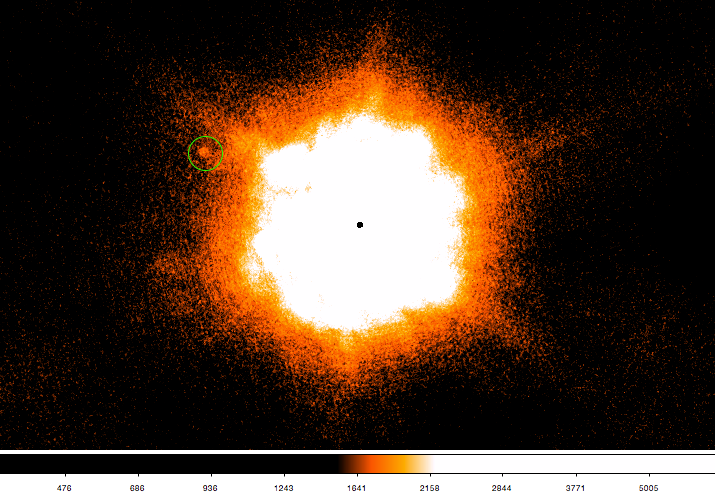
\includegraphics[width=\textwidth]{median}
  \caption{Median Combined Image for HR8799 system. On this image,
    only HR8799 b is clearly shown.}
  \label{fig:median}
\end{figure}
\subsection{Contrast Curve}
The procedure to make the contrast curve is described as following.
\begin{enumerate}
\item Add unsaturated PSFs  into original un-rotated images as fake
  planets. Fake planets are evenly placed 0 to 3 arcsec away from the
  peak of the primary star. A median combination of images with fake
  planets is presented in Figure \ref{fig:median_fakeplanet}. The peak
  value of the fake planet is fixed, and defined as
  $\mathrm{Amp_{PSF}}$
  
   \begin{figure}
    \centering
    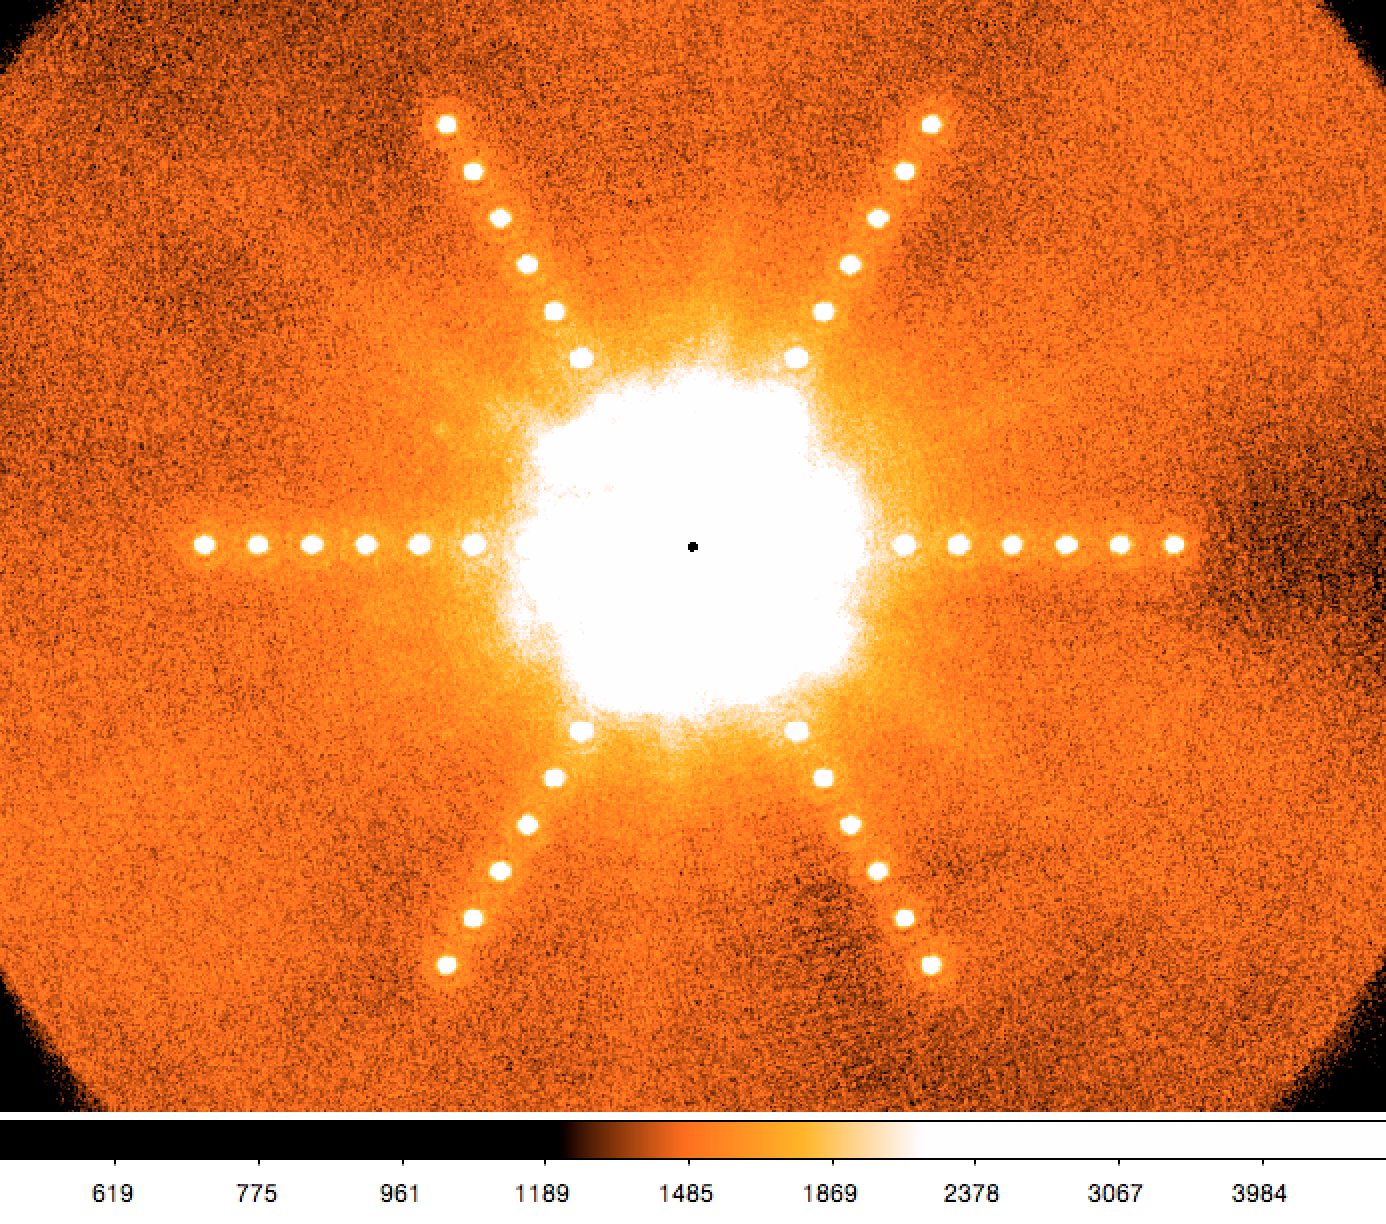
\includegraphics[width=\textwidth]{median_fake}
    \caption{Median combination of images with fake planets adding
      in. }
    \label{fig:median_fakeplanet}
  \end{figure}
 \item Noise is measured in an annulus around the  fake planet. The
   inner and outer radii of the annulus are 15 and 20 pixels. I define
   the noise as the square root of the second moment of the pixel
   values in the annulus to avoid negative value due to Primary
   subtraction.
   \[
     \mathrm{Noise} = \sqrt{\frac{1}{n}\sum_{i=1}^{n}F_{n}^{2}}
     \]
 \item S/N is defined as peak value of PSF   $\mathrm{Amp_{PSF}}$ and
   the Noise calculated as above. Contrast curve is defined as the
   relationship of S/N and angular separation. Figure
   \ref{fig:median_curve} presents the contrast curve for median
   combined image with   $\mathrm{Amp_{PSF}} = 2000$.
 \end{enumerate}

 \begin{figure}
   \centering
   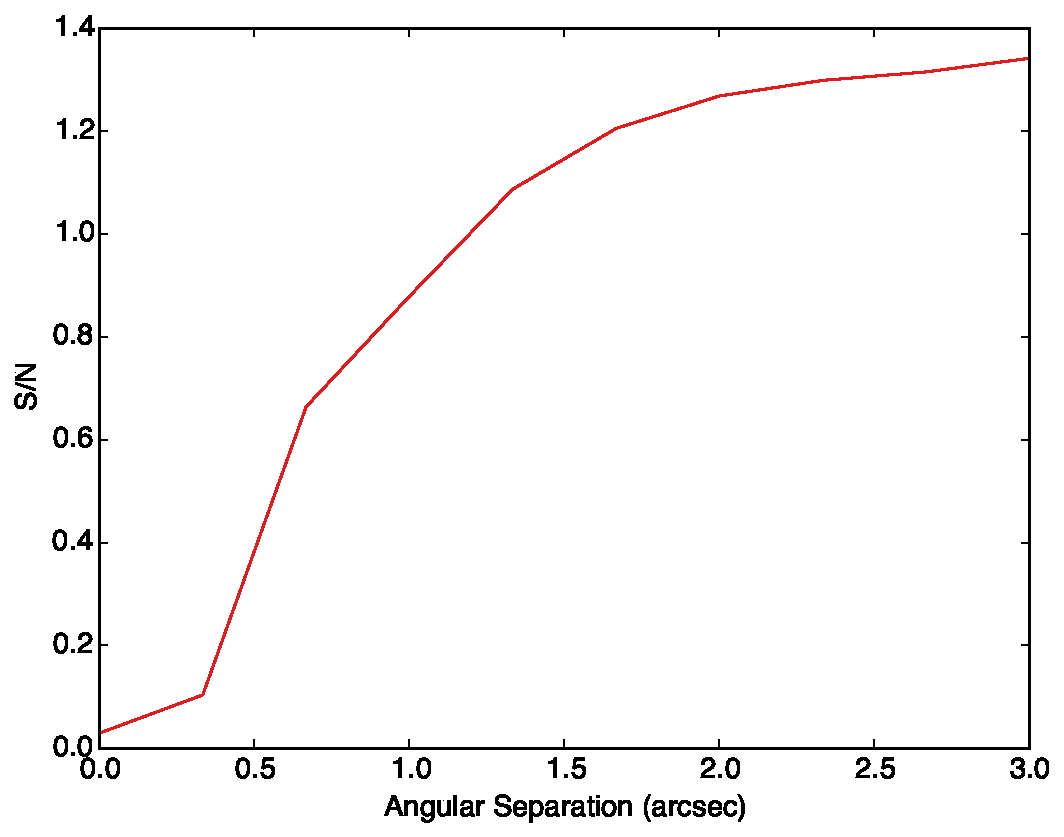
\includegraphics[width=\textwidth]{median_contrastCurve_amp=2000}
   \caption{Contrast curve for meian combined image. The PSF that used
     as fake planet is scaled so that the peak value is equal to
     2000. }
   \label{fig:median_curve}
 \end{figure}
 
\section{ADI}
\begin{figure}[!h]
  \centering
  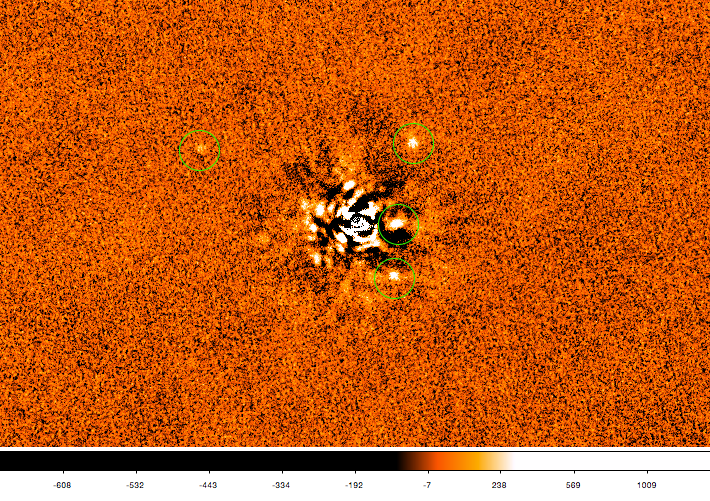
\includegraphics[width=\textwidth]{simple_ADI}
  \caption{HR8799 primary star subtracted with ADI technique. HR8799b,
    c, d now are clearly shown on the image. The bright spot near
    HR8799e is hardly tell whether it is the image of HR8799e or it is
    a quasi bright speckle.}
  \label{fig:simple_adi}
\end{figure}

   \begin{figure}
    \centering
    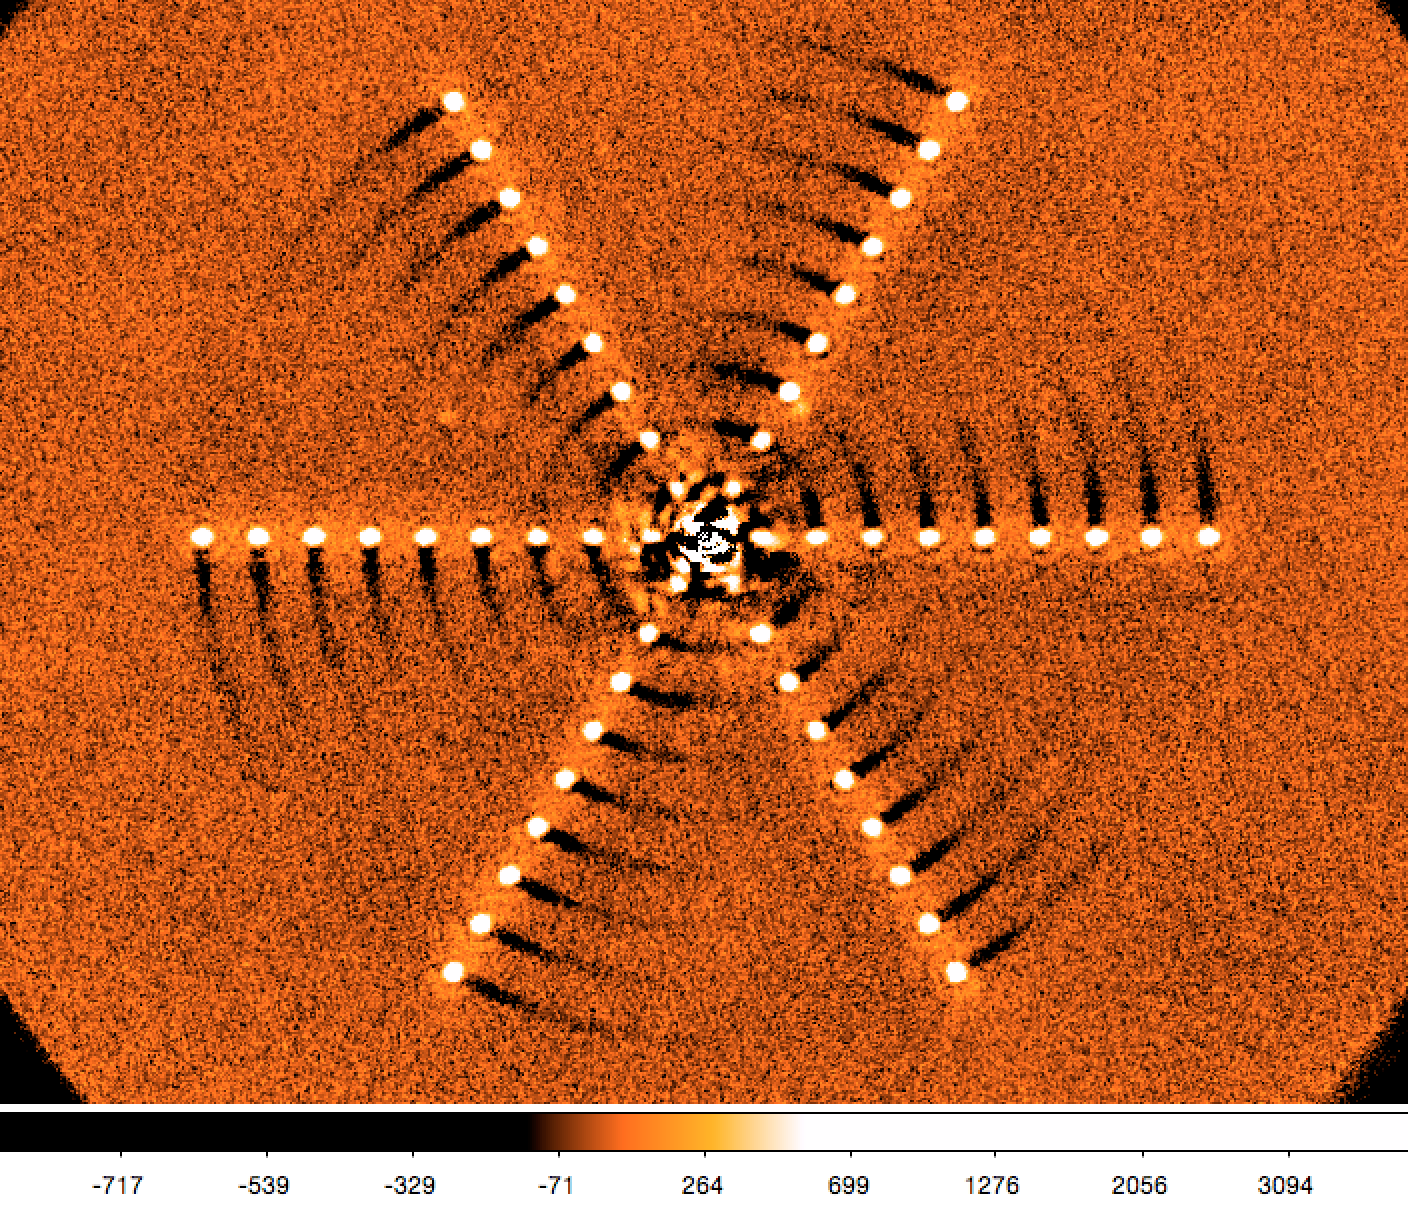
\includegraphics[width=\textwidth]{adi_fake}
    \caption{Image with primary subtracted using ADI with fake planets adding
      in.}
    \label{fig:adi_fakeplanet}
  \end{figure}

  \begin{figure}
   \centering
   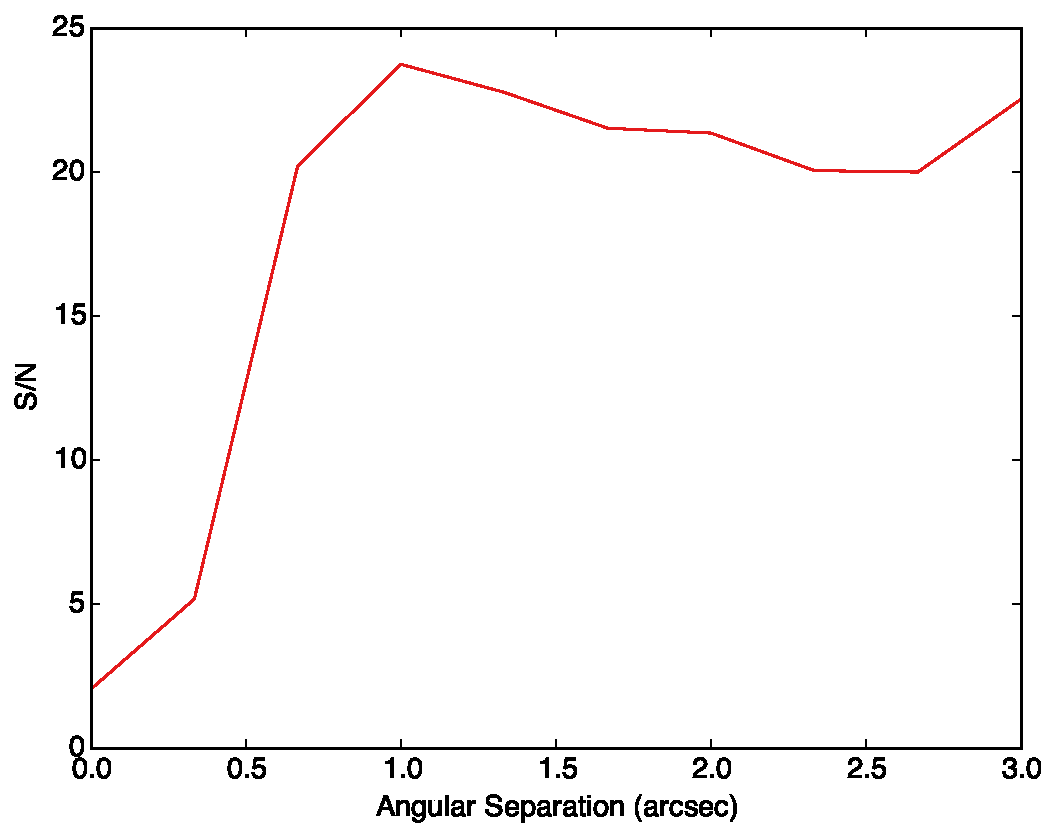
\includegraphics[width=\textwidth]{adi_contrastCurve_amp=2000}
   \caption{Contrast curve for image that is shown in Figure
     \ref{fig:adi_fakeplanet} . The PSF that used as fake planet is
     scaled the same way as in Figure \ref{fig:median_fakeplanet}}
   \label{adi:median_curve}
 \end{figure}
  
\end{document}
%%% Local Variables:
%%% mode: latex
%%% TeX-master: t
%%% End:
